\documentclass[conference, twocolumn]{IEEEtran}

\usepackage[utf8]{inputenc}
\usepackage[T1]{fontenc}
\usepackage{amsmath, amssymb}
\usepackage{graphicx}
\usepackage{listings}
\usepackage{xcolor}
\usepackage{hyperref}
\usepackage{booktabs}
\usepackage{float}

% Code listing style
\lstset{
  language=Python,
  basicstyle=\ttfamily\scriptsize,
  keywordstyle=\color{blue}\bfseries,
  commentstyle=\color{gray}\itshape,
  stringstyle=\color{red},
  breaklines=true,
  frame=single,
  numbers=left,
  numberstyle=\tiny\color{gray},
  columns=fullflexible,
  keepspaces=true
}

\title{Aerial Robotics Kharagpur Documentation\\Task 2.2 -- Image Cleaning and Denoising}

\author{Parv Chopra *}

\begin{document}

\maketitle

% ============================================================================
%  ABSTRACT
% ============================================================================
\begin{abstract}
This report documents the solutions to Tasks~2.2.1 and~2.2.2, both centred on image processing and noise removal. Task~2.2.1 addresses cleaning a noisy binary image of Iron Man: after an initial attempt using a custom $5\times5$ weighted-average kernel with Canny edge removal and a line prediction pipeline, the final approach uses Otsu's binarisation with connected-component cluster pruning to produce a clean binary image. Task~2.2.2 tackles denoising a heavily corrupted colour image: a comprehensive noise analysis characterises the corruption as additive, independent, Gaussian noise with $\sigma\approx63$, after which five standard denoising algorithms (Gaussian blur, bilateral filter, non-local means, channel-wise YCrCb denoising, and BM3D) were tried as initial attempts, and a custom BFS-based edge-aware blur was developed as the final approach. These tasks demonstrate classical image-processing techniques applicable to perception pipelines in aerial robotics and computer vision.
\end{abstract}

% ============================================================================
%  I. INTRODUCTION
% ============================================================================
\section{Introduction}

Task~2.2 comprises two sub-tasks in the domain of image processing:

\begin{itemize}
    \item \textbf{Task 2.2.1 -- Image Cleaning:} Given a noisy grayscale image (\texttt{iron\_man\_noisy.jpg}), clean it to recover the underlying structure as a clear binary image.
    \item \textbf{Task 2.2.2 -- Noise Analysis \& Image Denoising:} Given a heavily corrupted colour image (\texttt{noisy.jpg}), characterise the noise statistically and apply multiple denoising algorithms to recover the original image.
\end{itemize}

The challenge in both tasks is balancing noise removal with structure preservation --- aggressive filtering removes noise but also destroys thin lines and fine details, while gentle filtering leaves residual noise that degrades downstream processing.

% ============================================================================
%  II. PROBLEM STATEMENT
% ============================================================================
\section{Problem Statement}

\subsection{Task 2.2.1}
Given a noisy grayscale image:
\begin{enumerate}
    \item \textbf{Clean} the image to produce a clear binary representation of the underlying lines/shapes.
\end{enumerate}

\subsection{Task 2.2.2}
Given a noisy colour image:
\begin{enumerate}
    \item \textbf{Analyse} the noise to determine its type, distribution, standard deviation, and spectral characteristics.
    \item \textbf{Denoise} the image using multiple methods.
    \item \textbf{Compare} the denoising methods and identify the most effective approach.
    \item \textbf{Implement} a custom edge-aware denoising method that preserves structural edges.
\end{enumerate}

% ============================================================================
%  III. RELATED WORK
% ============================================================================
\section{Related Work}

\textbf{Gaussian/Median filtering} are standard noise-removal approaches. Gaussian filtering smooths uniformly; median filtering preserves edges better but can remove thin structures~\cite{opencv}.

\textbf{Otsu's thresholding}~\cite{opencv} automatically selects a binarisation threshold by minimising intra-class variance, and is effective when the histogram is bimodal.

\textbf{Connected-component analysis} labels contiguous regions; it is useful for removing small noise clusters by area~\cite{opencv}.

\textbf{Hough Line Transform}~\cite{opencv} maps edge points to $(\rho, \theta)$ parameter space to detect lines. The probabilistic variant (\texttt{HoughLinesP}) detects line segments directly.

\textbf{Bilateral Filter}~\cite{opencv} is an edge-preserving filter that weights pixels by both spatial distance and colour similarity.

\textbf{Non-Local Means}~\cite{opencv} compares patches across the entire image and averages similar ones, providing excellent detail preservation for Gaussian noise.

\textbf{BM3D} groups similar patches into 3D arrays and applies transform-domain collaborative filtering. It is widely considered the best classical denoiser.

% ============================================================================
%  IV. INITIAL ATTEMPTS
% ============================================================================
\section{Initial Attempts}

\subsection{Task 2.2.1 -- Image Cleaning}

\subsubsection{Method 1 -- Custom Kernel Filtering + Canny Edge Removal}

A hand-designed $5\times5$ weighted-average kernel was applied to smooth the image. The kernel emphasises neighbouring pixels while de-weighting the centre pixel (centre weight $= 0$):

\begin{equation}
K = \frac{1}{25} \begin{bmatrix} 0 & 1 & 1 & 1 & 0 \\ 1 & 1.25 & 2 & 1.25 & 1 \\ 1 & 2 & 0 & 2 & 1 \\ 1 & 1.25 & 2 & 1.25 & 1 \\ 0 & 1 & 1 & 1 & 0 \end{bmatrix}
\end{equation}

The zero centre weight means the output at each pixel depends entirely on its neighbours, providing aggressive smoothing. This was followed by binary thresholding at intensity~90, and Canny edge detection whose detected edges were removed (set to~0) to clean up boundary artefacts from the thresholding step.

\textbf{Result:} Produced a clean binary image but lost thin line details due to the aggressive smoothing kernel.

\subsubsection{Attempt 2 -- Line Prediction using Hough Transform}

After cleaning with Method~1, a line prediction pipeline was attempted. Canny edge detection (thresholds 50, 150) extracted edge pixels, and \texttt{cv2.HoughLinesP} (threshold~50, min length~30\,px, max gap~10\,px) detected line segments. Each segment was extended to the image boundaries, and morphological dilation ($5\times5$, 2 iterations) followed by closing ($5\times5$, 2 iterations) attempted to fill gaps. A morphological thinning algorithm was then applied to iteratively peel away boundary pixels until only single-pixel-wide skeletons remained.

\textbf{Result:} The pipeline detected 192 line segments and produced filled/thinned outputs, but the results were unsatisfactory --- the aggressive smoothing from Method~1 combined with line extension introduced artefacts, and the morphological gap filling distorted the original structure rather than recovering it.

\subsection{Task 2.2.2 -- Noise Analysis}

Before denoising, a comprehensive noise analysis was performed (\texttt{noise\_analysis.py}):

\begin{enumerate}
    \item \textbf{Global per-channel statistics}: Mean and standard deviation of each B, G, R channel across the entire image.
    \item \textbf{Flat-patch noise estimation}: Automatically detected the flattest $32\times32$ region (lowest local standard deviation) and measured noise $\sigma$ in that patch.
    \item \textbf{Channel correlation}: Computed inter-channel Pearson correlation coefficients of the noise residuals.
    \item \textbf{Distribution analysis}: Fitted a Gaussian distribution to the noise histogram.
    \item \textbf{Additive vs.\ multiplicative test}: Compared noise $\sigma$ in bright vs.\ dark regions. Constant $\sigma$ indicates additive noise; $\sigma$ scaling with intensity indicates multiplicative noise.
    \item \textbf{Frequency analysis (FFT)}: Computed the power spectrum of the noise. A flat spectrum confirms white noise.
\end{enumerate}

\textbf{Key findings:}
\begin{itemize}
    \item Noise is \textbf{additive} (constant $\sigma$ regardless of region brightness).
    \item Noise is \textbf{independent} across channels (low inter-channel correlation).
    \item Noise is approximately \textbf{Gaussian} (good histogram fit, skewness $\approx 0$, kurtosis $\approx 0$).
    \item $\sigma \approx 63$ per channel (very heavy).
    \item Noise is \textbf{spectrally white} (flat FFT).
\end{itemize}

\textbf{Conclusion:} The noise model is i.i.d.\ Gaussian $\mathcal{N}(0, 63)$ added independently to each R, G, B channel --- the classic AWGN model.

\subsection{Task 2.2.2 -- Trial Denoising Methods}

Five standard denoising methods were tried before developing the final custom approach:

\subsubsection{Method A -- Gaussian Blur}
A simple low-pass filter: a $21\times21$ box blur followed by two passes of $7\times7$ Gaussian blur. Very fast but blurs edges. Used as a baseline.

\subsubsection{Method B -- Bilateral Filter}
Edge-preserving filter with parameters $d=9$, $\sigma_{\text{color}}=75$, $\sigma_{\text{space}}=75$. Weights pixels by both spatial distance and colour similarity. Better edge preservation than Gaussian blur but slower.

\subsubsection{Method C -- Non-Local Means}
Patch-based denoising: \texttt{cv2.fastNlMeansDenoisingColored} with $h=30$, template window $5\times5$, search window $21\times21$. Compares patches across a search area and averages similar ones. Followed by a light $3\times3$ Gaussian blur to smooth residual artefacts.

\subsubsection{Method D -- YCrCb Channel-wise Denoising}
Converts to YCrCb colour space to exploit human perceptual sensitivity:
\begin{itemize}
    \item \textbf{Y} (luminance): denoised lightly ($h=6$) to preserve detail.
    \item \textbf{Cr, Cb} (chrominance): denoised aggressively ($h=15$) since the human eye is less sensitive to colour noise.
\end{itemize}
Each channel is processed independently with \texttt{fastNlMeansDenoising}, then merged and converted back to BGR.

\subsubsection{Method E -- BM3D}
Block-Matching and 3D Filtering: the state-of-the-art classical denoiser. The image is normalised to $[0,1]$, and BM3D is applied per channel with $\sigma_{\text{psd}} = 63/255 \approx 0.25$. Groups similar patches into 3D arrays and applies transform-domain shrinkage.

\textbf{Result:} While BM3D and NL-Means produced strong results numerically, none of these methods provided strict edge preservation --- they all blur edges to some degree. This motivated the development of the custom edge-aware blur as the final approach.

% ============================================================================
%  V. FINAL APPROACH
% ============================================================================
\section{Final Approach}

\subsection{Task 2.2.1 -- Image Cleaning}

The final approach uses Otsu's binarisation followed by connected-component cluster removal (\texttt{final\_otsu\_cleanup.py}):

\textbf{Step 1 -- Otsu's Automatic Thresholding:} The noisy grayscale image is binarised using Otsu's method~\cite{opencv}. Otsu's algorithm works by examining the histogram of pixel intensities and finding the threshold value that minimises the weighted sum of variances within the two classes (foreground and background). For every possible threshold $t \in [0, 255]$, it splits the pixels into two groups --- those below $t$ and those above --- computes the variance within each group, and selects the $t$ that minimises the combined intra-class variance:
\begin{equation}
    t^* = \arg\min_t \bigl[\omega_0(t)\,\sigma_0^2(t) + \omega_1(t)\,\sigma_1^2(t)\bigr]
\end{equation}
where $\omega_0, \omega_1$ are the class probabilities and $\sigma_0^2, \sigma_1^2$ are the class variances. This automatically adapts to the image's histogram without manual threshold tuning.

\textbf{Step 2 -- Connected-Component Analysis:} All contiguous regions are labelled using 8-connectivity (including diagonal neighbours).

\textbf{Step 3 -- Small Cluster Removal:} Any connected component with fewer than~7 pixels is removed (set to~0). This eliminates isolated noise speckles --- which are typically small and disconnected --- while preserving genuine line segments and shapes, which form larger contiguous regions.

\textbf{Output:} \texttt{method2\_cleaned.jpg} --- a clean binary image of the Iron Man drawing with noise removed and structure preserved.

\begin{figure}[H]
\centering
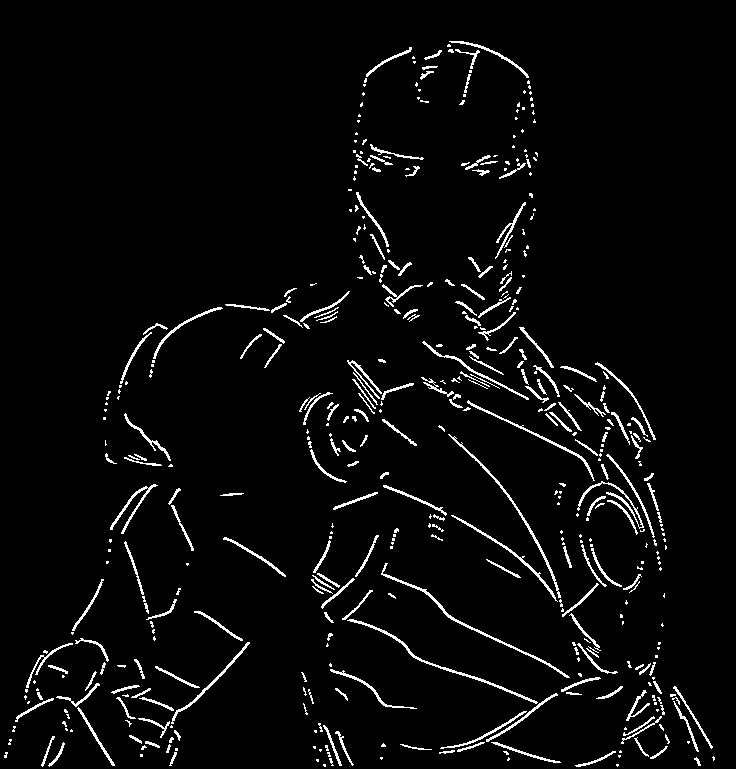
\includegraphics[width=0.9\columnwidth]{Task_2.2.1/method2_cleaned.jpg}
\caption{Task 2.2.1 final output: cleaned binary image after Otsu binarisation and cluster removal.}
\label{fig:method2_cleaned}
\end{figure}

\subsection{Task 2.2.2 -- Custom Edge-Aware Blur}

The final approach for denoising is a fully custom edge-aware blur implementation (\texttt{final\_edge\_aware\_blur.py}) consisting of:

\begin{enumerate}
    \item \textbf{Edge detection}: Multi-scale Sobel gradients with non-maximum suppression and hysteresis thresholding --- a complete edge detector implemented from scratch without using \texttt{cv2.Canny}.
    \item \textbf{BFS flood-fill blur}: For each non-edge pixel, BFS explores a kernel-sized window. The flood \emph{cannot cross edge pixels}, so only reachable non-edge pixels on the same side of the edge contribute to the average. This ensures edges are never blurred across.
    \item \textbf{Edge pixel inpainting}: Edge pixels are iteratively filled from their non-edge neighbours (outside-in), preventing black edge artefacts in the output.
\end{enumerate}

Key parameters:
\begin{table}[H]
\centering
\begin{tabular}{@{}lrl@{}}
\toprule
\textbf{Parameter} & \textbf{Default} & \textbf{Description} \\
\midrule
\texttt{EDGE\_PRE\_BLUR} & 15 & Gaussian blur before edges \\
\texttt{SOBEL\_KSIZE} & 9 & Sobel kernel size \\
\texttt{LOW\_PCT} & 75 & Lower hysteresis percentile \\
\texttt{HIGH\_PCT} & 85 & Upper hysteresis percentile \\
\texttt{EDGE\_DILATE} & 1 & Edge dilation in pixels \\
\texttt{BLUR\_KERNEL} & 7 & BFS blur window size \\
\texttt{BLUR\_ITERS} & 3 & Number of blur passes \\
\bottomrule
\end{tabular}
\end{table}

\begin{figure}[H]
\centering
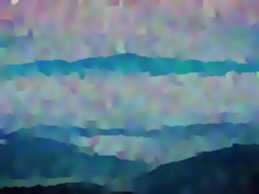
\includegraphics[width=0.9\columnwidth]{Task_2.2.2/edge_aware_blur.jpg}
\caption{Task 2.2.2 final output: edge-aware blur result.}
\label{fig:edge_aware_blur}
\end{figure}

% ============================================================================
%  VI. RESULTS AND OBSERVATION
% ============================================================================
\section{Results and Observation}

\subsection{Task 2.2.1}

Two cleaning methods were compared. Method~1 (custom kernel + Canny) produced a binary image but lost thin line details due to the aggressive smoothing. The subsequent line prediction pipeline (Hough Transform + morphological gap filling + thinning) introduced further artefacts rather than improving the result.

The final approach --- Otsu binarisation + connected-component cluster removal --- produced significantly better results. Otsu's automatic threshold selection adapts to the image histogram, and the connected-component pruning targets isolated noise speckles specifically rather than blurring globally. The output (\texttt{method2\_cleaned.jpg}) is a clean binary image preserving the underlying line structure.

\subsection{Task 2.2.2}

Table~\ref{tab:denoise_comparison} summarises all denoising methods tried.

\begin{table}[H]
\centering
\caption{Comparison of denoising methods on a noisy image with $\sigma \approx 63$.}
\label{tab:denoise_comparison}
\begin{tabular}{@{}lcccc@{}}
\toprule
\textbf{Method} & \textbf{Speed} & \textbf{Edges} & \textbf{Noise} & \textbf{Overall} \\
\midrule
A. Gaussian     & Fast   & Poor      & Good      & Baseline \\
B. Bilateral    & Medium & Good      & Medium    & Better   \\
C. NL-Means     & Slow   & Very Good & Very Good & Strong   \\
D. YCrCb        & Slow   & Very Good & Very Good & Strong   \\
E. BM3D         & Slow   & Excellent & Excellent & Strong   \\
\textbf{Custom BFS} & \textbf{V. Slow} & \textbf{Excellent} & \textbf{Good} & \textbf{Final} \\
\bottomrule
\end{tabular}
\end{table}

The custom BFS edge-aware blur was selected as the final approach because it provides strict edge preservation --- edges are never blurred across, unlike all other methods which blur edges to varying degrees. While Methods~A--E produced varying levels of noise removal, they all compromise edge sharpness. The BFS approach guarantees that the blur window cannot cross detected edges, making it the most structurally faithful denoiser despite its higher computational cost.

\begin{figure}[H]
\centering
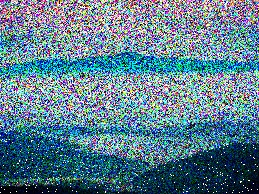
\includegraphics[width=0.9\columnwidth]{Task_2.2.2/noisy.jpg}
\caption{Original noisy input image ($\sigma \approx 63$).}
\label{fig:noisy_input}
\end{figure}

% ============================================================================
%  VII. FUTURE WORK
% ============================================================================
\section{Future Work}

\subsection{Task 2.2.1}
\begin{itemize}
    \item \textbf{Adaptive cluster-size threshold}: The minimum cluster size (currently fixed at~7) could be optimised per image based on noise statistics.
    \item \textbf{Multi-scale Otsu}: Applying Otsu at multiple resolutions and combining results could improve robustness for images with varying noise density.
    \item \textbf{Deep learning denoising}: A trained denoising autoencoder could outperform hand-crafted thresholding on complex noise patterns.
\end{itemize}

\subsection{Task 2.2.2}
\begin{itemize}
    \item \textbf{Deep learning denoisers}: Trained models (DnCNN, FFDNet, Restormer) can outperform classical methods, especially at high noise levels.
    \item \textbf{Automatic noise-level estimation}: Automatic $\sigma$ estimation from the image would make the pipeline fully automatic.
    \item \textbf{GPU acceleration}: The BFS-based edge-aware blur is extremely slow. A GPU implementation or approximation using guided filtering could achieve similar results orders of magnitude faster.
    \item \textbf{Blind denoising}: Methods that work without knowing $\sigma$ (e.g.\ noise2noise, self2self) would be more practical in real-world scenarios.
\end{itemize}

% ============================================================================
%  CONCLUSION
% ============================================================================
\section*{Conclusion}

This report presented solutions to two image-processing tasks. For Task~2.2.1, two cleaning approaches were tried --- custom kernel filtering with Canny edge removal (followed by an unsuccessful line prediction pipeline), and Otsu's binarisation with connected-component cluster pruning. The latter was adopted as the final approach, providing clean noise removal while preserving the underlying line structure.

For Task~2.2.2, a comprehensive noise analysis pipeline confirmed the noise as additive, independent, Gaussian with $\sigma \approx 63$ and spectrally white. Five standard denoising methods (Gaussian blur, bilateral filter, non-local means, YCrCb channel-wise, and BM3D) were tried as initial approaches. The final solution is a custom edge-aware blur using BFS flood-fill, which guarantees strict edge preservation during denoising by preventing the blur window from crossing detected edges.

\textit{Acknowledgement:} Rudraksh Gupta supported during the development and debugging of this project.

% ============================================================================
%  REFERENCES
% ============================================================================
\begin{thebibliography}{9}

\bibitem{opencv}
OpenCV, ``OpenCV Documentation,'' \url{https://docs.opencv.org/}, accessed 2025.

\end{thebibliography}

\end{document}
